\documentclass[10pt, a4paper]{exam}
\usepackage{graphicx}
\usepackage[a4paper, total={7in, 9.5in}]{geometry}
\usepackage[normalem]{ulem}
\usepackage{amsmath}
\renewcommand\ULthickness{1.0pt}   
\setlength\ULdepth{1.3ex}

\begin{document}


	\noindent
	\begin{minipage}[l]{0.1\textwidth}
		\noindent
		
\includegraphics[width=2.8\textwidth]{ESCUDO.png}
	\end{minipage}
\hfill
\begin{minipage}[c]{0.8\textwidth}
	\begin{center}
		{\large  Departamento de Ingeniería civil y Agrícola\par
		\large	Facultad de Ingeniería	\par
	% \large \textbf{Taller propiedades de los fluidos}	\par
    \large \textbf{Laboratorio No. 1 \\ Resalto Hidráulico}	\par
} Prof. Luis Alejandro Morales, Ph.D.
	\end{center}
\end{minipage}
\par
\vspace{0.2in}
\noindent
    \uline{Estructuras hidráulicas [2015954]	\hfill 2024-II	}
\par 
\vspace{0.15in}
\noindent

%%%%%%%%%%%%%%%%%%%%%%%%%%%%%
\section{Normas del Laboratorio}
\begin{itemize}
    \item \textbf{Grupos}: Los grupos serán de 5 o 6 estudiantes máximo. Los estudiantes son libres de organizar los grupos.
    
    \item \textbf{Duración}: Cada grupo tendrá una hora aproximadamente para realizar el laboratorio.
    
    \item \textbf{Material}: Es necesario vestir bata u overol para la realización del laboratorio. Este atuendo puede ser de cualquier color o fabricante. Traer calculadora, lápiz y papel.
\end{itemize}


\section{Objetivo}

En términos generales, este laboratorio tiene como fin estudiar el flujo gradualmente variado (FGV) y el comportamiento del resalto hidráulico. A continuación algunos objetivos específicos:

\begin{itemize}

    \item Calcular y dibujar los perfiles de flujo generado antes y desp\'ues del resalto bajo las condiciones impuestas. Comparar los resultados mediante la medición experimental de las profundidades con el limnímetro.
    
    \item Calcular el perfil teórico con un valor de manning de $n=0.009$ (valor aproximado para el materia del canal), aplicando métodos de cálculo de $FGV$ cómo el método del paso estándar para encontrar el perfil. Para esto es necesario tambi\'en hallar el valor de la profundidad crítica y normal.
    
    \item Comparar los perfiles obtenidos en los dos literales anteriores y en caso de diferir, ajustar el n de manning para que los perfiles coincidan, luego consultar en la literatura a que material correspondería dicho coeficiente.

    \item Realizar el análisis del resalto respecto a las profundidades subsecuentes y la longitud del resalto.
    
\end{itemize}


\section{Metodología}

Se dispondrá de un canal rectangular horizontal de paredes de vidrio de $31cm$ de ancho, dicho canal se alimenta mediante un tanque de aquietamiento que esta  conectado a una tubería proveniente de un tanque de nivel constante. El caudal que transporta el canal se regula mediante una válvula colocada en la tubería (ver figuras ~\ref{fig:esqpdf} y ~\ref{fig:esqreal}).

\begin{figure}[h]
    \centering
    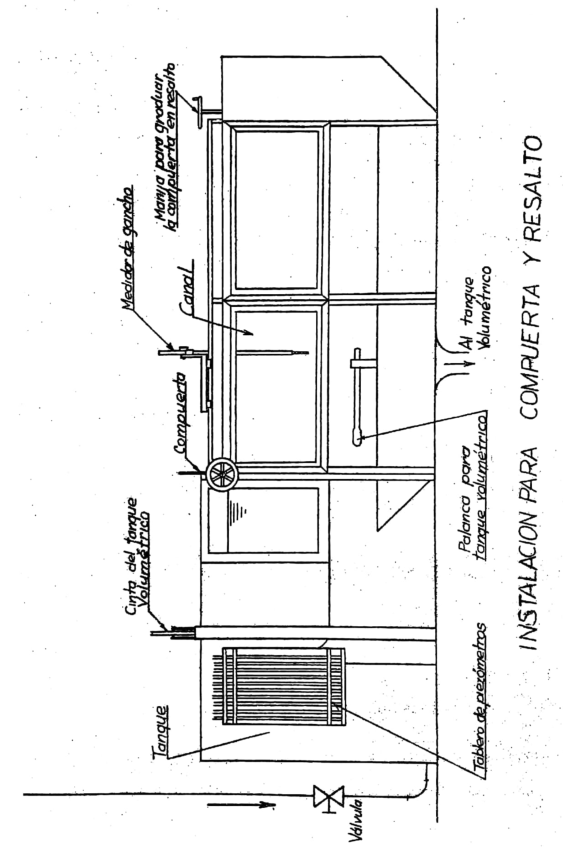
\includegraphics[angle=270,width=0.75\linewidth]{Images/esquema.png}
    \caption{Esquema general de la instalación.}
    \label{fig:esqpdf}
\end{figure}

\begin{figure}[h]
    \centering
    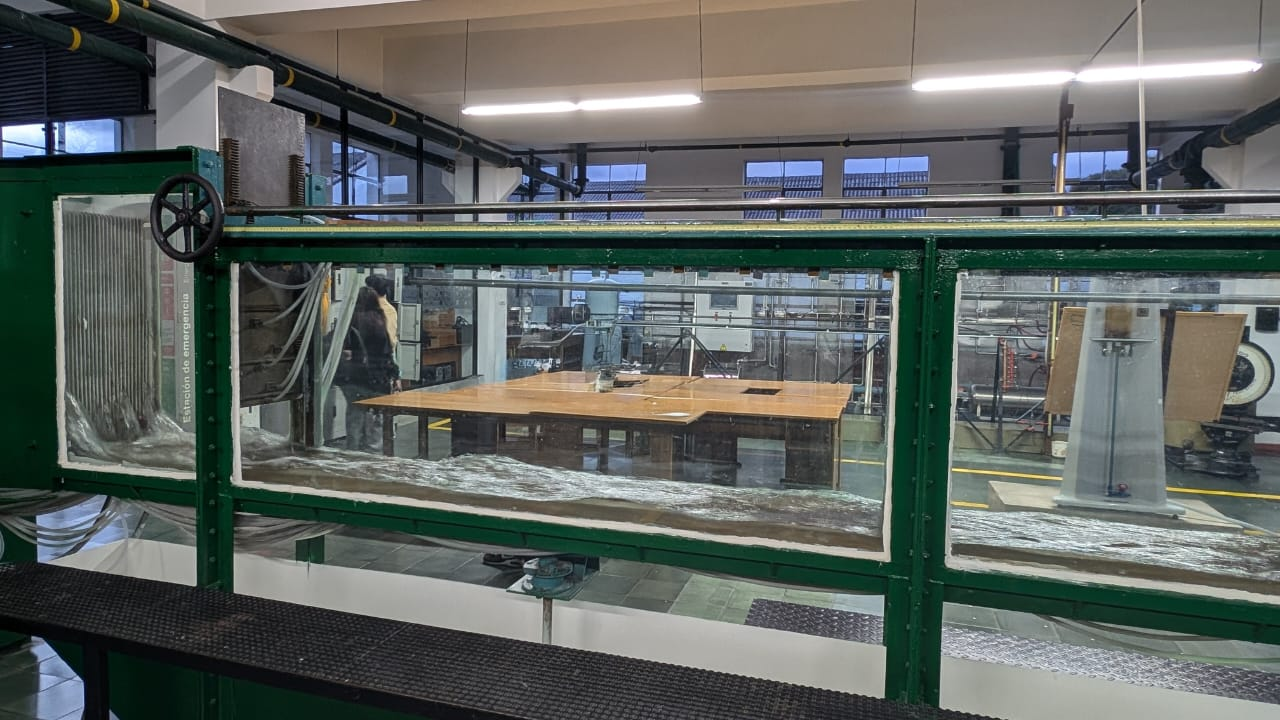
\includegraphics[width=0.75\linewidth]{Images/real.jpg}
    \caption{Canal dispuesto en el edificio de hidráulica.}
    \label{fig:esqreal}
\end{figure}

El tanque volumétrico será utilizado para el cálculo del caudal que pasar\'a por la compuerta. Este valor se conoce midiendo el desplazamiento de la cinta y el tiempo que transcurre en dicho desplazamiento (Figura \ref{fig:cinta}). 

\begin{figure}[h]
    \centering
    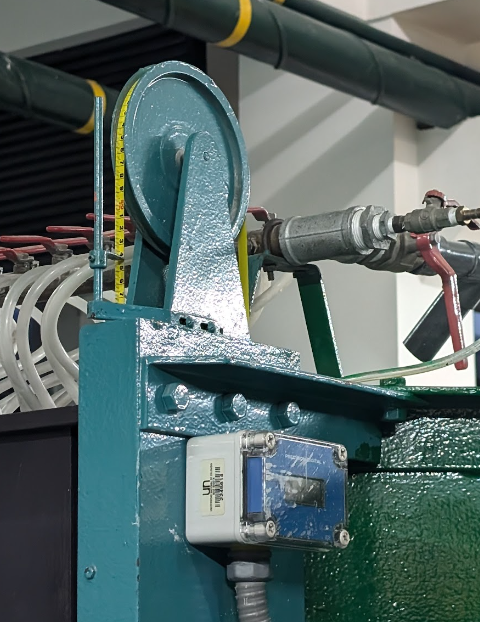
\includegraphics[width=0.19\linewidth]{Images/cinta.png}
    \caption{Cinta para la medición del caudal.}
    \label{fig:cinta}
\end{figure}

%\newpage

A lo largo del canal se encuentra un limnímetro montado en un riel desplazable. Este instrumento será el que permitirá las medidas de las profundidades a lo largo del canal. El esquema de este montaje se muestrar en la figura~\ref{limni}.

\begin{figure}[h]
    \centering
    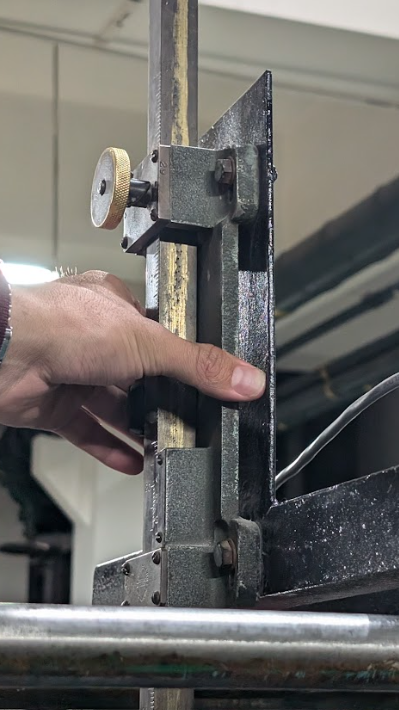
\includegraphics[width=0.25\linewidth]{Images/limnimetro.png}
    \caption{Limnímetro a utilizar para la medición de la lámina de agua.}
    \label{limni}
\end{figure}

Para producir y controlar el resalto hidráulico se debe manipular la manija que se encuentra al final del canal (de izquierda a derecha) en la parte superior, con el fin de graduar la compuerta dispuesta al final del canal. 

Para el caso de las mediciones con el limnímetro considerar un cero de 5.2 cm a la salida de la primera compuerta (aguas arriba) y un cero de 4.8 cm al final del canal (aguas abajo). Las profundidades de flujo se obtienen restando el cero (calculado de acuerdo con la distancia) al valor medido con el limnímetro.


%\newpage


\section{Ecuaciones y resultados}


\begin{enumerate}

    \item Para la medición del caudal, se toma una medición inicial con la cinta (fig \ref{fig:cinta}), y luego una final después de 90 segundos, luego la resta entre estas dos mediciones corresponderá a la medición del tanque; se recomienda tomar 4 de estas mediciones y promediarlas, de modo qué:

    $$dif.alturas_1=med_{t=0s}-med_{t=90s}=alt.final_{1}$$

    Teniendo en cuenta que el tanque es de $2.2m$ por $7.1m$ se tendrá:

    $$Q (m^3/s)=\dfrac{(2.2m\cdot 7.1m \cdot (prom.alt.final) m)}{90seg}$$
    
    \item Se toma una valor inicial de $y$ y se realiza un solver con la expresión del número de Froude (cuando este es igual a 1) para encontrar la profundidad crítica $y_c$.

    $$Fr=\dfrac{Q}{\sqrt{g(A^3/T)}}$$

    O simplemente utilizando la expresión para un canal rectangular, donde $q$ es el caudal por unidad de ancho.

    $$y_c=\sqrt[3]{\dfrac{q^2}{g}}=\sqrt[3]{\dfrac{Q^2}{B^2 g}}$$
    
    \item Con los datos geométricos del canal y el valor de n de manning $(n=0.009)$, aplicar el método del paso estándar para encontrar el perfil, se recomienda utilizar un $\Delta x$ de $0.1m$ o $0.2m$.

    %$$y_{i+1}=y_{i}+\dfrac{1}{6}(k_1+2k_2+2k_3+k_4)\Delta x$$

    
    \item Aplicar las ecuaciones de profundidad subsecuente

    $$\dfrac{y_1}{y_2}=\dfrac{1}{2}\left(\sqrt{1+8Fr^2_2}-1\right)$$    

%\newpage

    $$\dfrac{y_2}{y_1}=\dfrac{1}{2}\left(\sqrt{1+8Fr^2_1}-1\right)$$
    
\item Hallar la longitud del resalto mediante la figura~\ref{resh}.

    \begin{figure}[h]
        \centering
        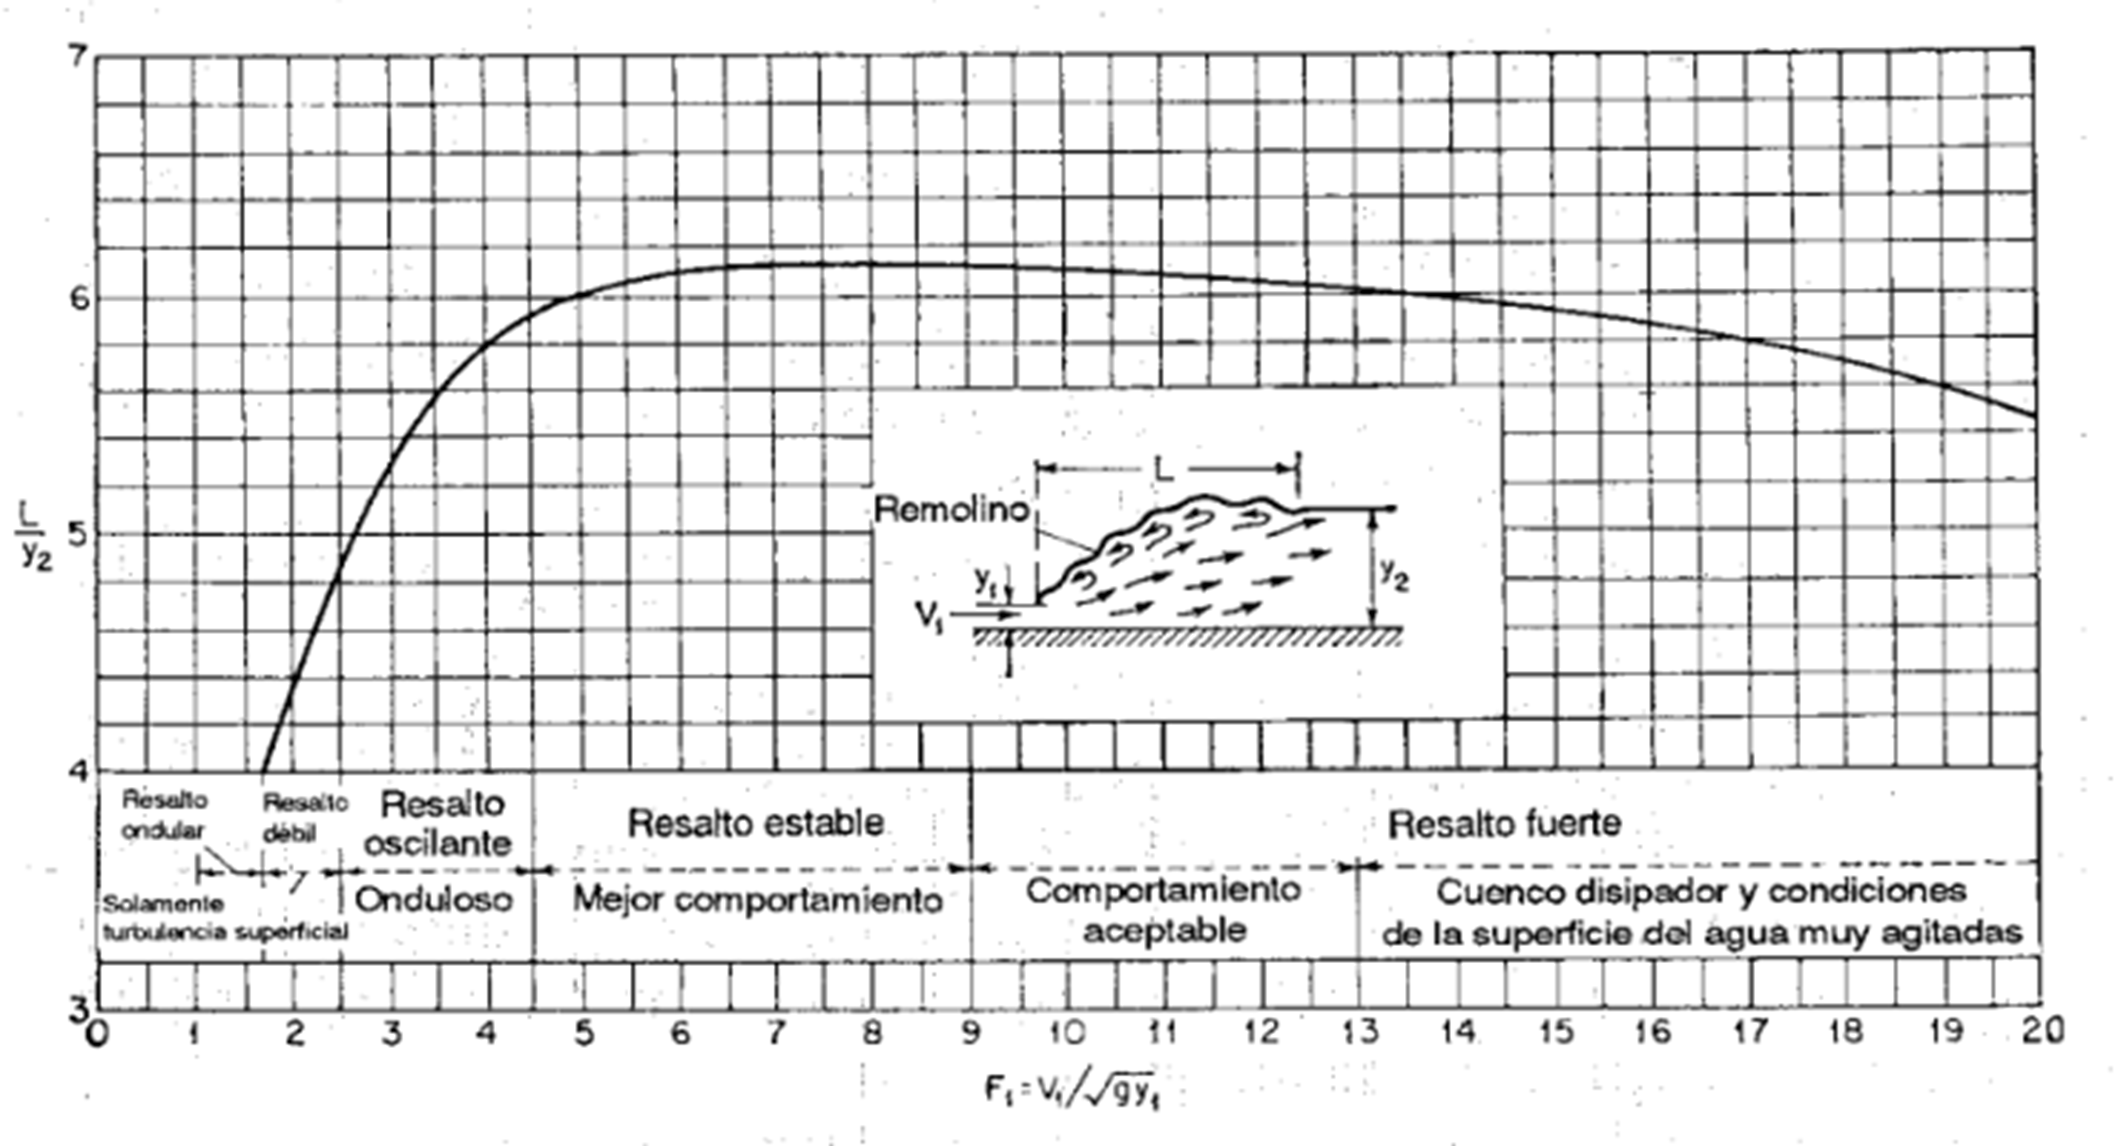
\includegraphics[width=0.9\linewidth]{Images/resalto.png}
        \caption{Relación entre las profundidades subsecuentes y la longitud del resalto.}
        \label{resh}
    \end{figure}

\item Comprobar si el valor tomado de la figura~\ref{resh} es similar al obtenido con la expresión:

    $$L=5(y_2-y_1)$$

    \item Comparar los perfiles trazados con los valores teóricos y experimentales. Ajustar el valor de $n$.

    \item Comparar los valores medidos con los calculados para el resalto hidr\'aulico.

    \item Discutir los resultados.
\end{enumerate}


\section{Listado de instrumentos usados}

\begin{enumerate}

    \item Medición de caudal:
    
        \begin{enumerate}
        
            \item \textbf{Tanque volumétrico:} Utilizado para medir el caudal.
            
        \end{enumerate}
        
    \item Medición y control de altura:
    
        \begin{enumerate}
        
            \item \textbf{Compuertas:} Utilizadas aguas arriba y aguas abajo del canal para regular el flujo.
            \item \textbf{Limnímetro:} Conjunto de reglas graduadas en centímetros que miden las variaciones del nivel de la superficie del agua.
            
        \end{enumerate}
        
\end{enumerate}

\section{Informe}

El informe de laboratorio debe contener las siguientes secciones:

\begin{enumerate}

    \item \textbf{Introducción:} Breve texto para poner en contexto el laboratorio.
    
    \item \textbf{Metodología:} Describe el procedimiento de toma de datos y el seguido para obtener los resultados (sustentar con algunas fotografías de ser posible).
    
    \item \textbf{Resultados y análisis:} Presenta los resultados del laboratorio. Dado el caso, se deben incluir gráficas y tablas que resuman los resultados.
    
    \item \textbf{Conclusiones:} Se discuten allí las conclusiones obtenidas a partir de los resultados. Se hacen las comparaciones del caso.
    
    \item \textbf{Referencias:} Incluir las referencias consultadas.
\end{enumerate}

\end{document}



